\documentclass[12pt,letterpaper]{article}
\usepackage{fullpage}
\usepackage[top=2cm, bottom=4cm, left=2.5cm, right=2.5cm]{geometry}
\usepackage{amsmath,amsthm,amsfonts,amssymb,amscd}
\usepackage{lastpage}
\usepackage{enumerate}
\usepackage{fancyhdr}
\usepackage{mathrsfs}
\usepackage{xcolor}
\usepackage{graphicx}
\usepackage{listings}
\usepackage{hyperref}
\usepackage{float}

\hypersetup{%
  colorlinks=true,
  linkcolor=blue,
  linkbordercolor={0 0 1}
}
 
\renewcommand\lstlistingname{Algorithm}
\renewcommand\lstlistlistingname{Algorithms}
\def\lstlistingautorefname{Alg.}

\lstdefinestyle{Python}{
    language        = Python,
    frame           = lines, 
    basicstyle      = \footnotesize,
    keywordstyle    = \color{blue},
    stringstyle     = \color{green},
    commentstyle    = \color{red}\ttfamily
}

\setlength{\parindent}{0.0in}
\setlength{\parskip}{0.05in}
\begin{document}






Foundations of Applied Math\\
 HW \#2
 Due Thursday 


\begin{enumerate}

\item 1.1) \#7
  \emph{Solution.} $a_{n}(1.005) + 500, a_{0} = 5000$
\item 1.2) \#2
  \emph{Solution.} 
  Plotting the data in Figure \ref{fig:1}, we can see the data follows an exponential pattern. 

  \begin{figure}[!htb]
    \center{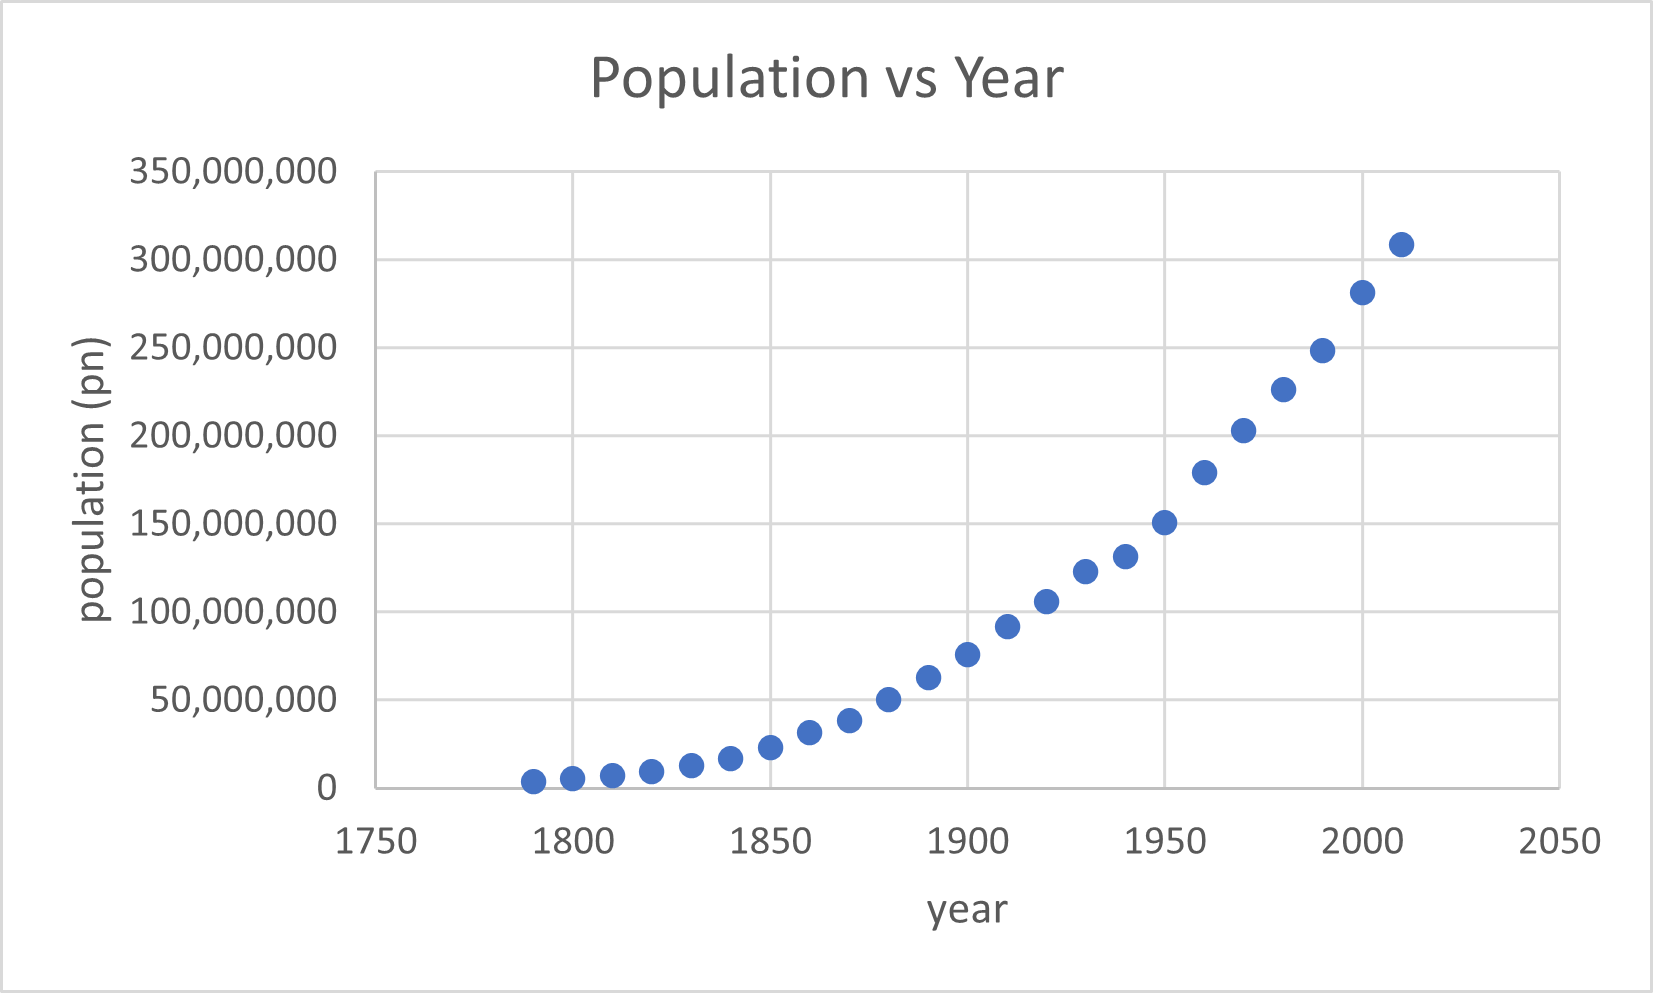
\includegraphics[scale=.9]{popvsyear.png}}
    \caption{\label{fig:1} Plot of the data given by the problem.}
  \end{figure}

  Exponential models can be modelled using the equation $\Delta pn = kpn$. To find
  the value of k, we can plot the $\Delta pn$ vs $pn$ graph and use the slope of that 
  graph to find k. 

  \begin{figure}[!htb]
    \center{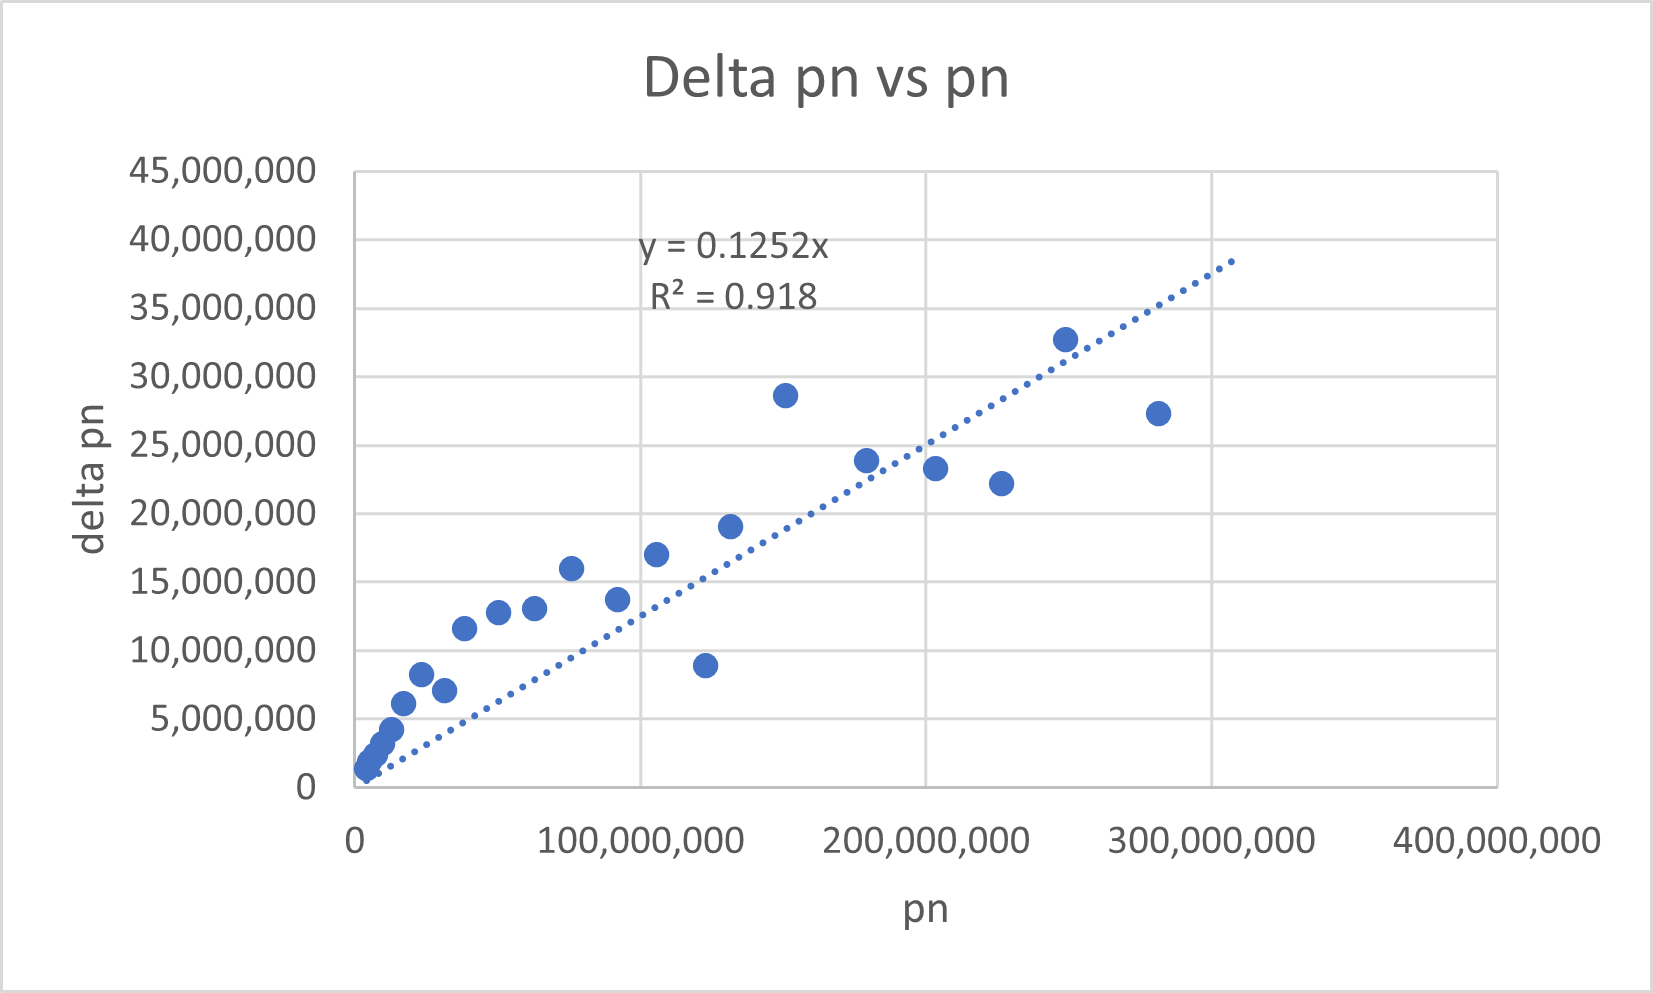
\includegraphics[scale=.9]{deltapnvspn.png}}
    \caption{\label{fig:2} Plot of $\Delta pn$ vs $pn$.}
  \end{figure}

  As our $R^2$ value is quite close to 1, we can confidently use the slope we found 
  in Figure \ref{fig:2} as our $k$ value giving us an exponential model of:
  \vskip1em
  \begin{center}
    $\Delta pn = .1252pn$\\
    $p_{n+1} - p_{n} = .1252p_{n}$\\
    $p_{n+1} = 1.1252p_{n}$
  \end{center}

  After iterating this model over the same amount of years given in the data, 
  we see the model plot in orange and the actual data in blue. 

  \begin{figure}[!htb]
    \center{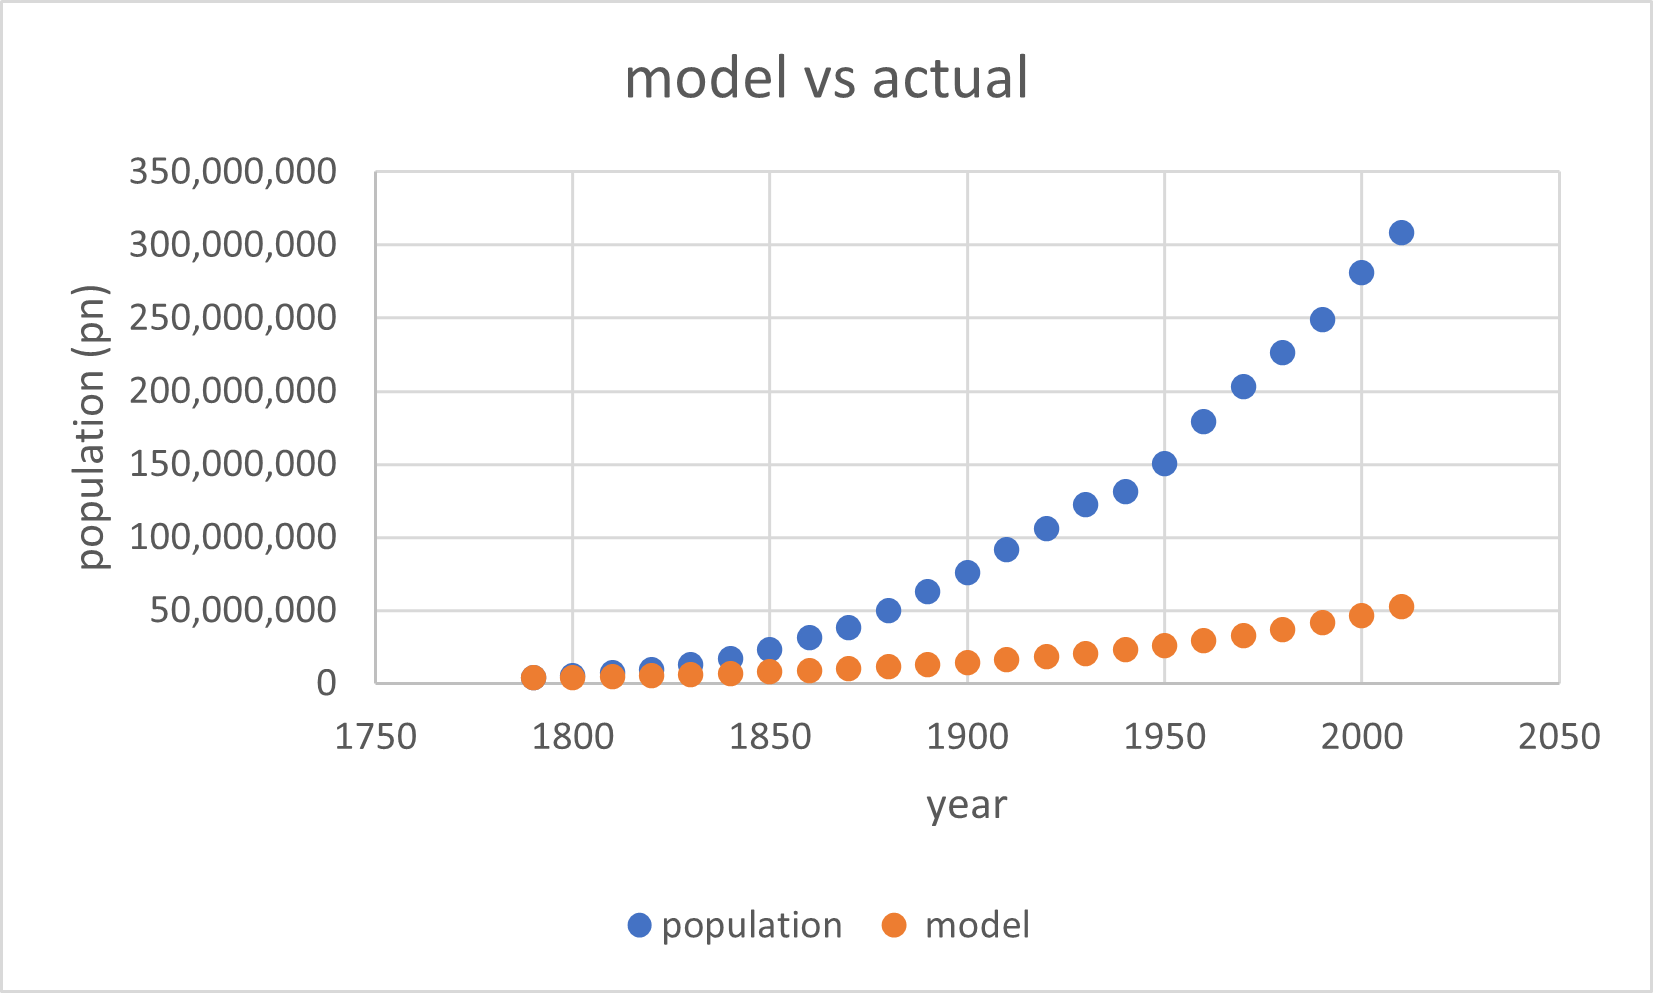
\includegraphics[scale=.9]{modelvsactual.png}}
    \caption{\label{fig:3} Plot of the model vs the actual data given.}
  \end{figure}

\pagebreak
\item 1.2) \#9
  \emph{Solution.} 
  \begin{enumerate}
    \item Plotting the graph, we see that there is a clear linear relationship between
          $\Delta a_{n}$ and $n$:

    \begin{figure}[!htb]
      \center{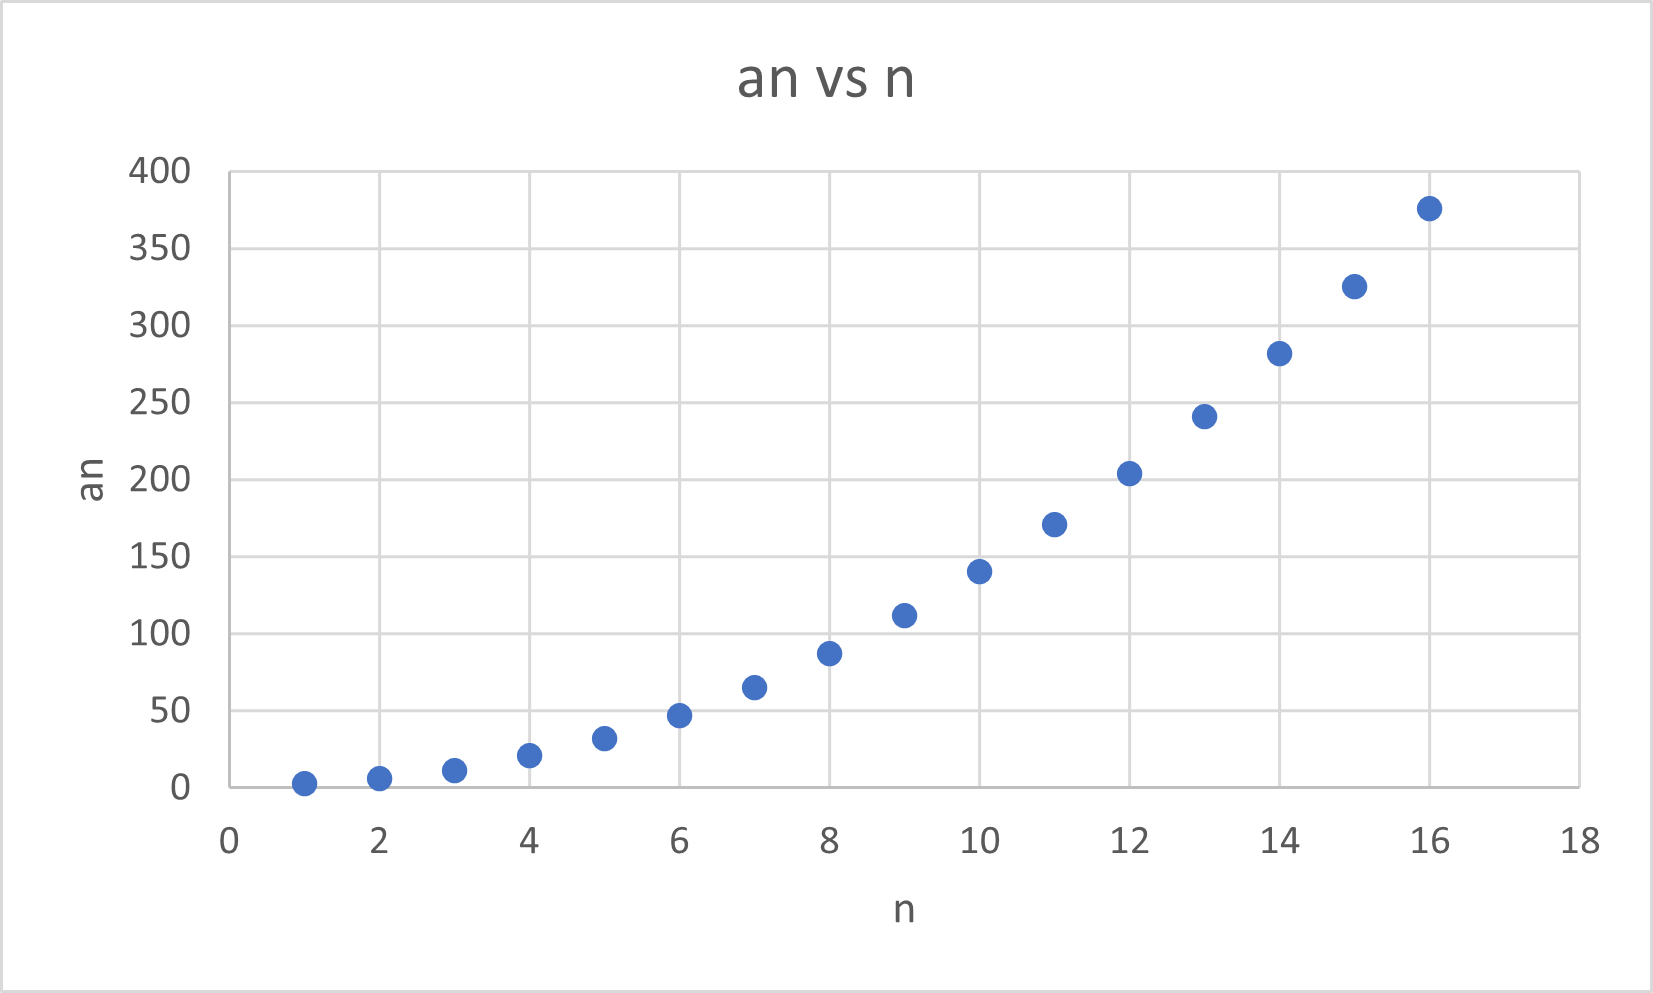
\includegraphics[scale=.9]{9 an vs n.png}}
      \caption{\label{fig:4} Plot of $\Delta pn$ vs $pn$.}
    \end{figure}

    \item Based on the graph of part (a), we know the $\Delta a_{n}$ vs $n$ graph is linear. 
          Using this information, we can find a difference equation of the form .
          $a_{n+1} = a_{n} + 3.1395n$
          Plotting the errors in the predicted values against n: 
      
    \begin{figure}[!htb]
      \center{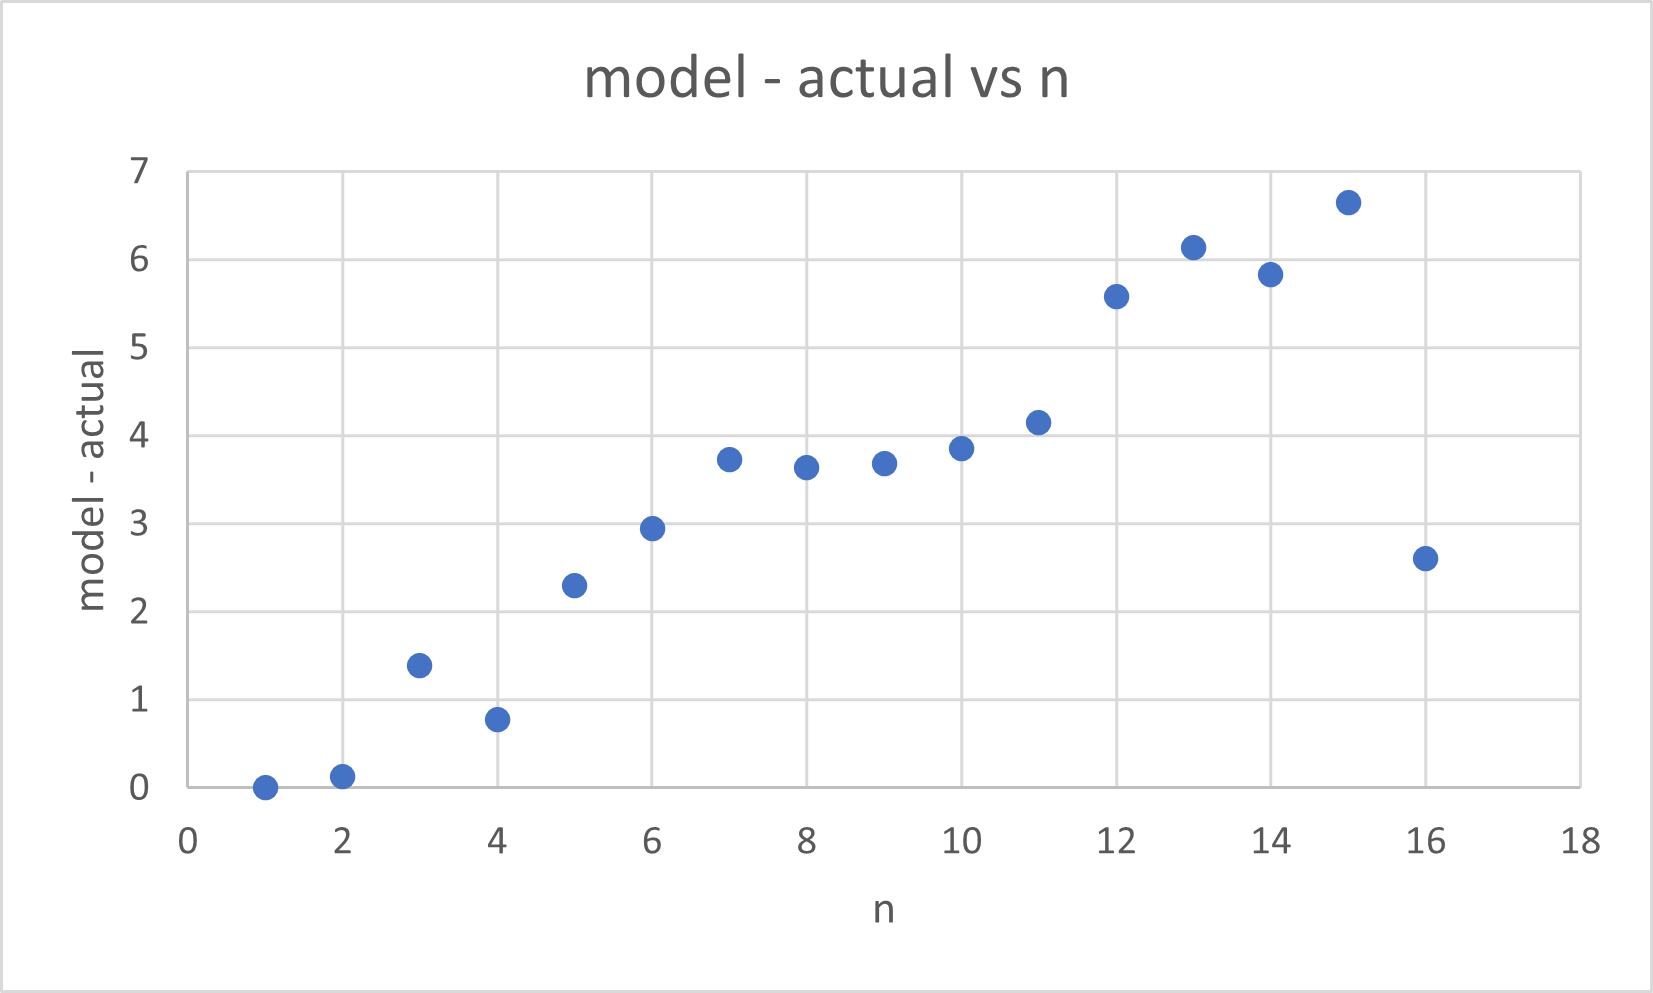
\includegraphics[scale=.9]{model actual difference.png}}
      \caption{\label{fig:5} Plot of the difference between the model and the actual data for every n.}
    \end{figure}
    Since the errors in the plotted graph in Figure \ref{fig:5} is quite small for every single data point, 
    we can see this model is appropriate and should accuately model the data given. 
  \end{enumerate}
\pagebreak

\item 1.3) \#1c
  \vskip1em
  \emph{Solution.}
  The solution for an equation in the form $a_{n+1} = ra_{n}$ is $a_{k} = r^ka_{0}$.\\
  So, substituting the values given to us, we get the solution: $a_{k} = (3/4)^k 64$
\item 1.3) \#1f
  \vskip1em 
  \emph{Solution.}
  Our solution is of the form $a_{k} = r^k c + \frac{b}{1-r}$
  By plugging in our values of $r$ and $b$, we get: 
  \begin{center}
    $a_{k} = (.1)^k c + \frac{3.2}{.9}$
    $a_{k} = (.1)^k c + \frac{32}{9}$
  \end{center}

  To this, we can plug in our initial condition, $a_{0} = 1.3$: 
  \begin{center}
    $1.3 = (.1)^0 c + \frac{32}{9}$ \\
    $1.3 = c + \frac{32}{9}$ \\
    $1.3 - \frac{32}{9} = c$\\
    $c \approx -2.256$
  \end{center}

  So, our solution to the equation takes the form: 
  \begin{center}
    $a_{k} = -2.256(.1)^k + \frac{32}{9}$
  \end{center}

\item 1.3) \#3a
  \vskip1em
  \emph{Solution.}
  From the given equation, we find that the equilibrium solution is: 
  \begin{center}
    $a_{0} = \frac{50}{2.2}$
  \end{center}

  However, because our $|r|$ value is greater than 1, we can conclude that our function
  will be unstable, as shown in Figure \ref{fig:6} below. 
  \begin{figure}[!htb]
    \center{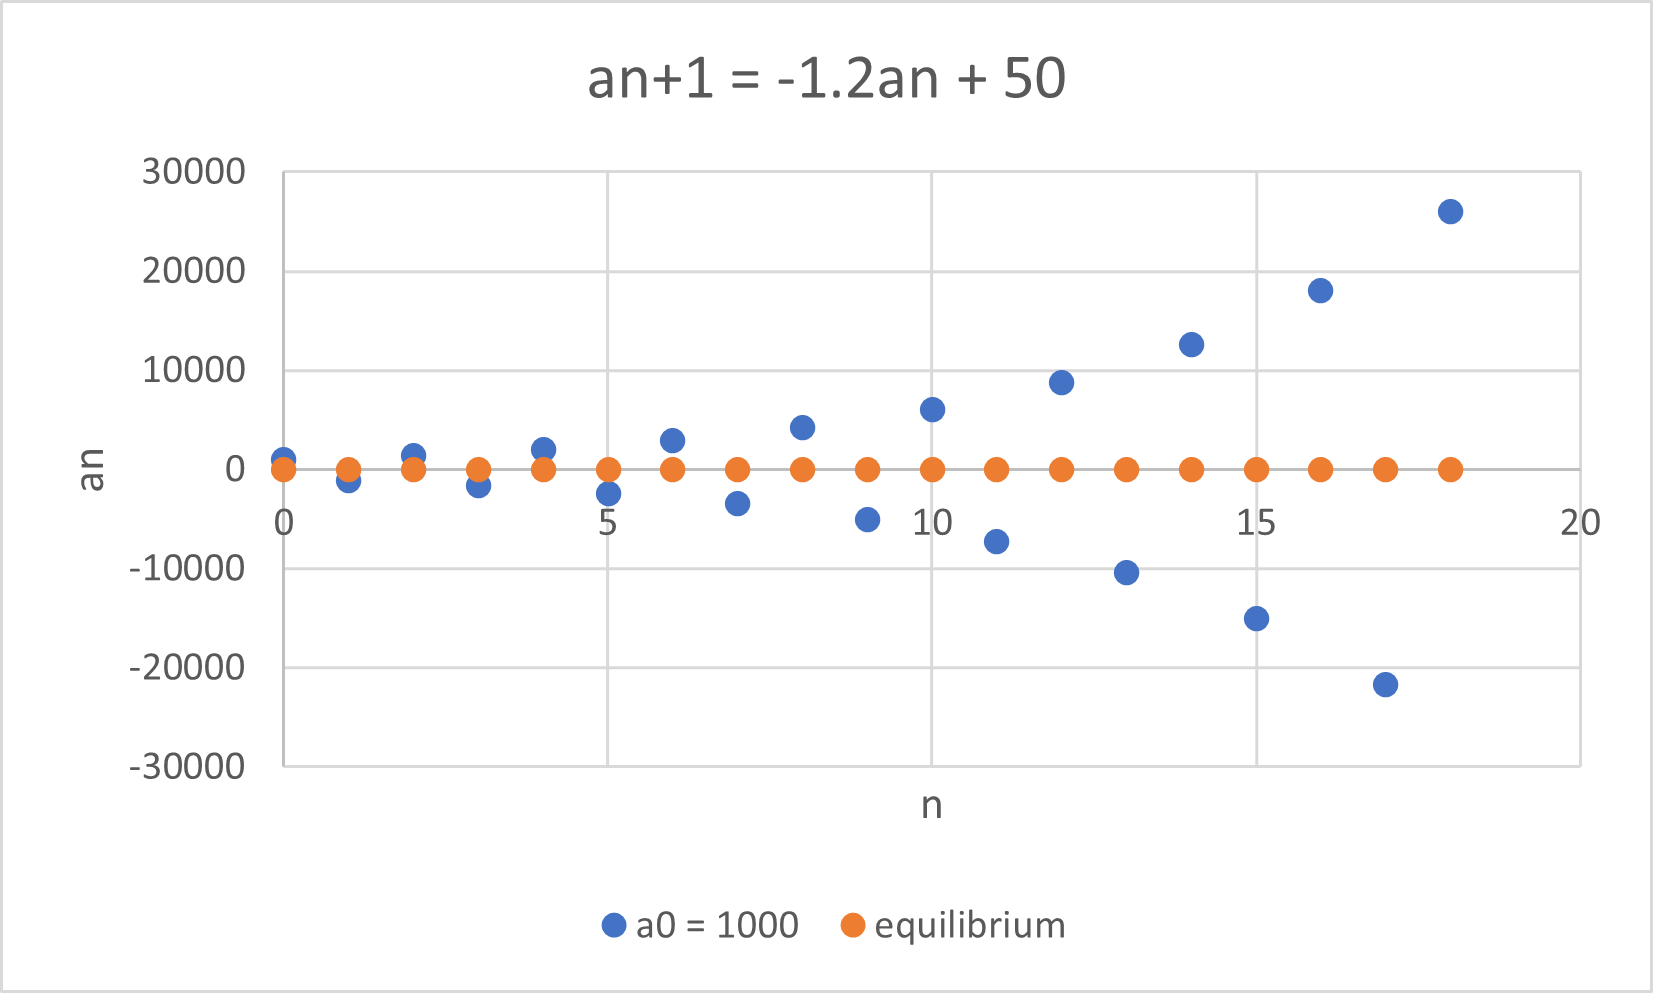
\includegraphics[scale=.9]{1.3 3a .png}}
    \caption{\label{fig:6} Plot of the model vs the actual data given.}
  \end{figure}

\pagebreak
\item 1.3) \#3c
  \vskip1em
  \emph{Solution.}
  From the given equation, we find the equilibrium solution is: 
  \begin{center}
    $a_{0} = -500$
  \end{center}
  which happens to be the same initial condition given to us by the problem.
  The $|r|$ value for our equation is less than one in this case, so we can conclude
  this will be a stable equilibrium as shown below.
  \begin{figure}[!htb]
    \center{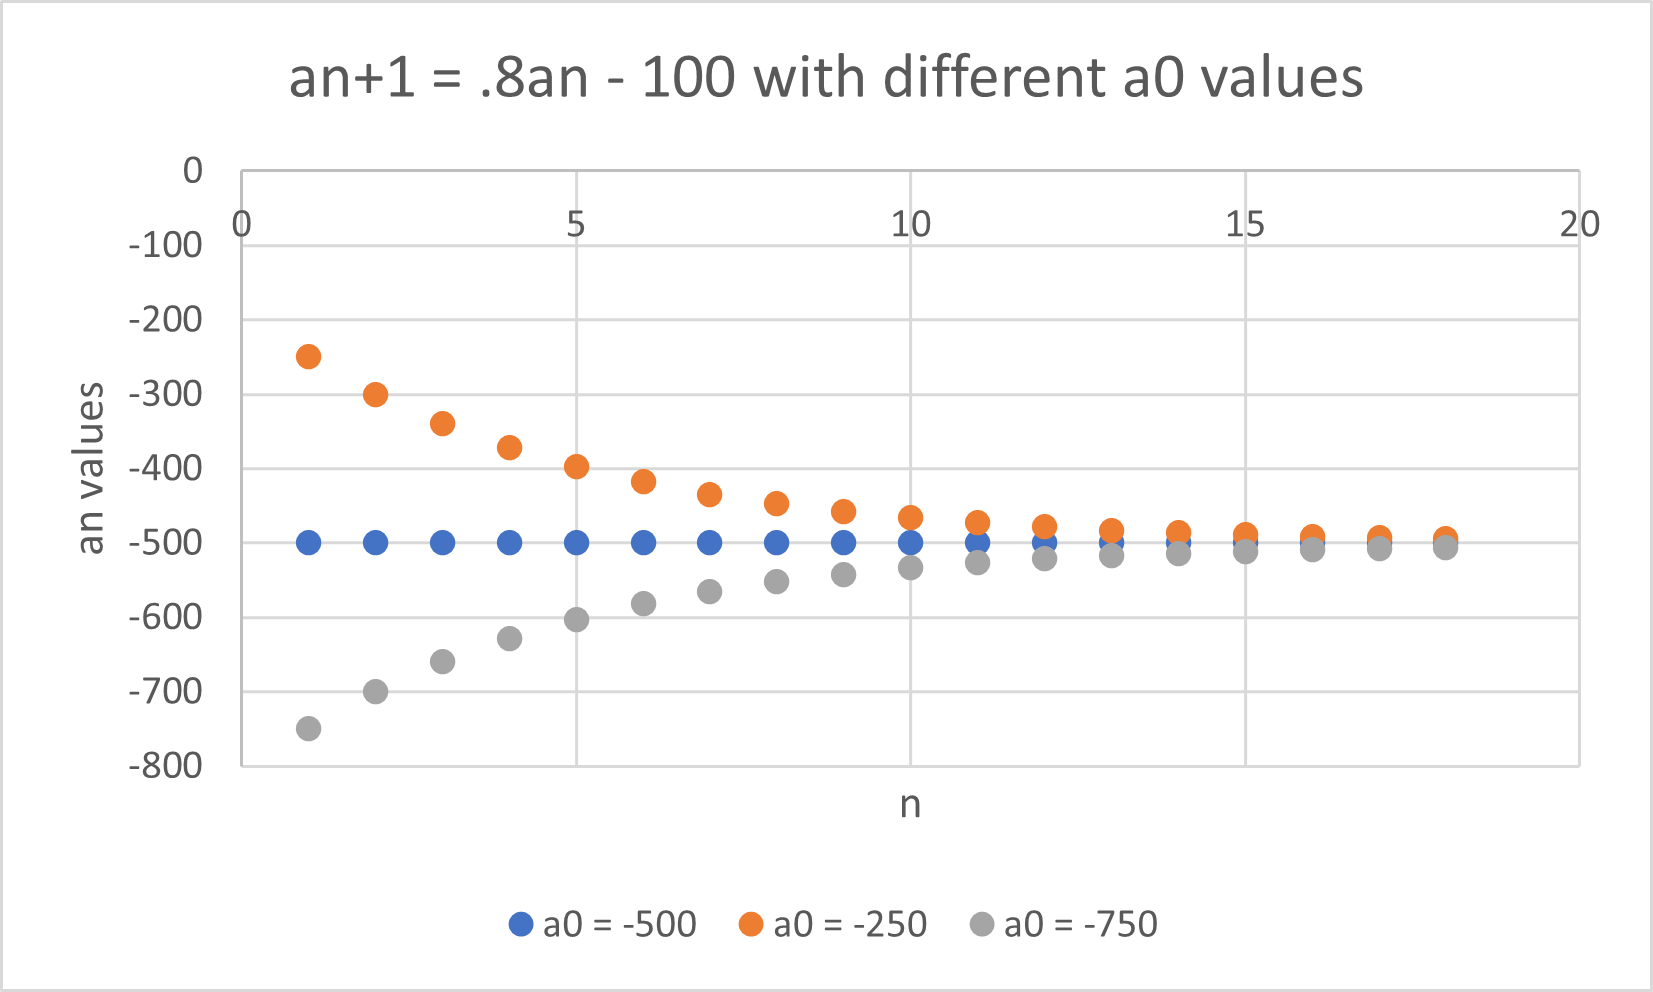
\includegraphics[scale=.9]{1.3 3c.png}}
    \caption{\label{fig:7} Plot of the model vs the actual data given.}
  \end{figure}

\item Suppose for a drug,  we have the following data where the values in rows 2 and 3 are in mg and the top row is in days.

\begin{tabular}{|l|l|l|l|l|l|l|l|l|l|}
\hline
$n$          & 0     & 1     & 2     & 3     & 4     & 5     & 6     & 7     & 8    \\ \hline
$a_n$        & .5    & .345  & .238  & .164  & .113  & .078  & .054  & .037  & .026 \\ \hline
$\Delta a_n$ & -.155 & -.107 & -.074 & -.051 & -.035 & -.024 & -.017 & -.011 &      \\ \hline
\end{tabular}

\noindent Formulate a model representing the amount of drug left in the body after $n$ days. Note this doesn't seem realistic you'll see!

\emph{Solution.}
Plotting the graph above, we see the drug decays exponentially
\begin{figure}[!htb]
  \center{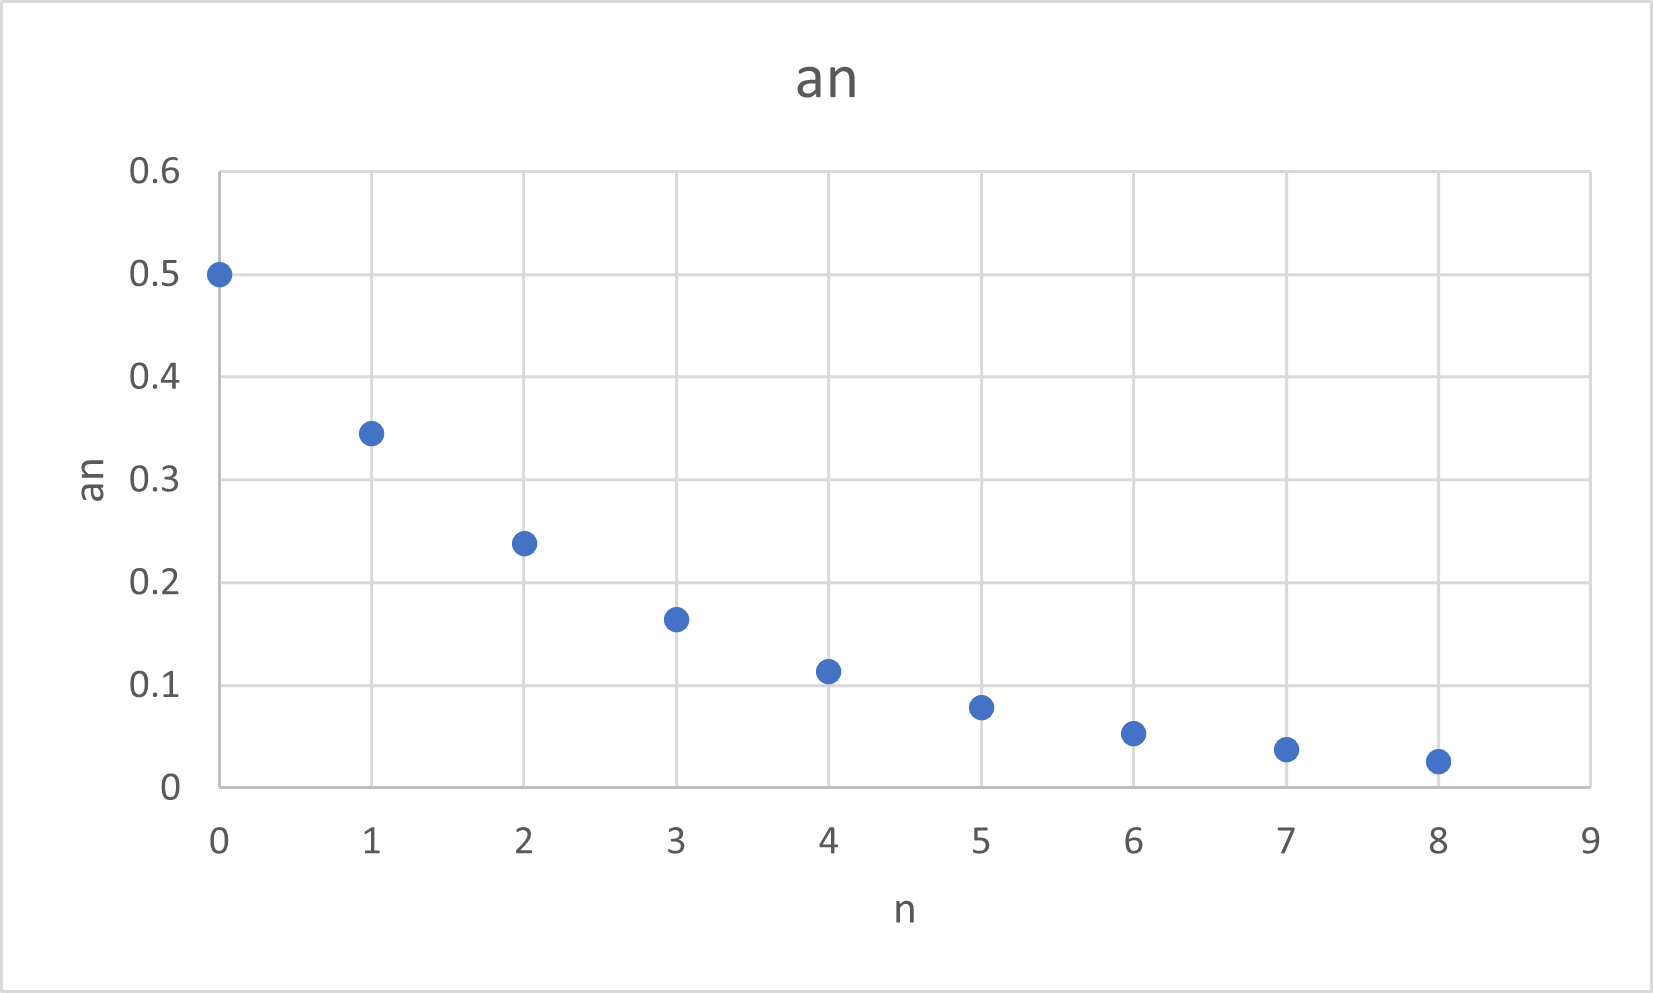
\includegraphics[scale=.8]{number8 an vs n.png}}
  \caption{\label{fig:8} Plot of $a_{n}$ vs $n$}
\end{figure}

So we can use the exponential difference equation $\Delta a_{n+1} = ka_{n}$. 
In order to find the value of $k$, we can plot the graph of $\Delta a_{n}$ vs $a_{n}$ 
of which the slope of the graph will be our value for $k$ which we have done below:
\begin{figure}[!htb]
  \center{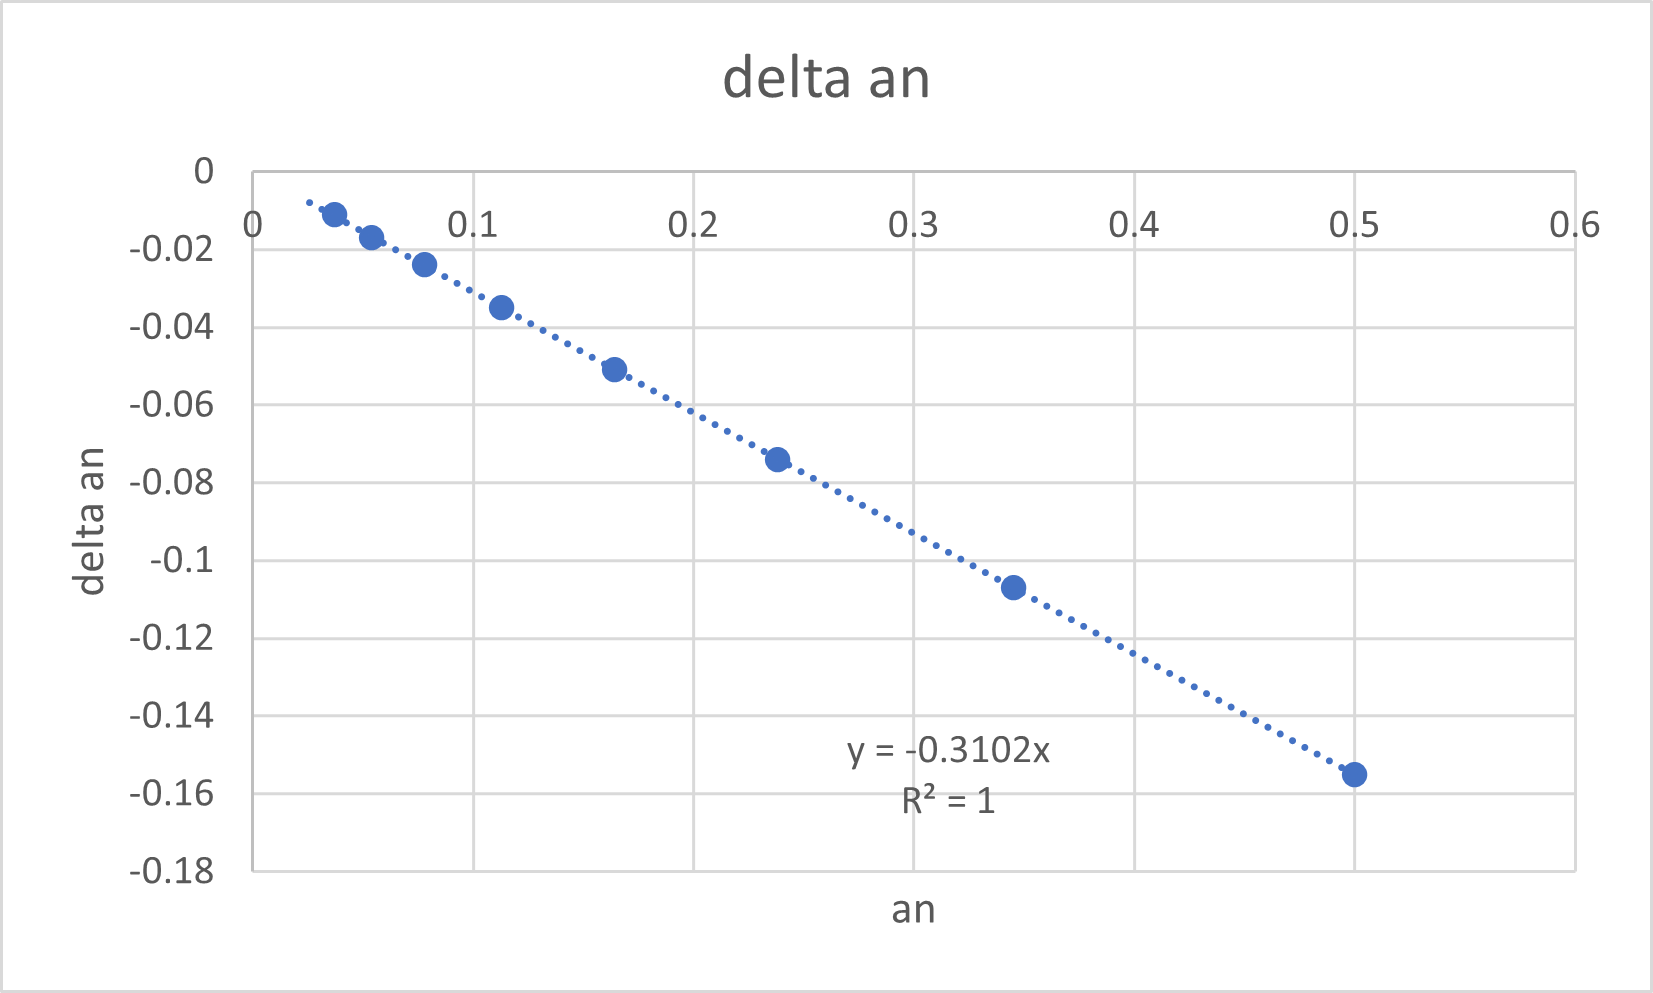
\includegraphics[scale=.8]{number8 delta an vs an.png}}
  \caption{\label{fig:9} Plot of $\Delta a_{n}$ vs $a_{n}$}
\end{figure}

Using the slope of Figure \ref{fig:9}, we derive our value for $k$ 
\begin{center}
  $k = -0.3102$
\end{center}
from which we get our difference equation:
\begin{center}
  $\Delta a_{n+1} = ka_{n}$\\
  $\Delta a_{n+1} = -0.3102a_{n}$\\
  $a_{n+1} - a_{n} = -0.3102a_{n}$\\
  $a_{n+1} = 0.6898a_{n}$
\end{center}

\item  Suppose for yet another drug we prescribe a daily drug dosage of 0.1 mg and know that half the drug remains in the system at the end of each dosage period.
\vskip1em
\noindent Write down a model to describe this.
\vskip1em
\emph{Solution.} $a_{n+1} = .5a_{n} + .1$
\vskip1em
\noindent 
 Given the three starting doses, 0.1, 0.2, and 0.3 (mg).
Is there a value in mg that the system will approach after a fews days for each of these three  initial dosages? \\
\emph{Solution.} 
From the model above, we can find the equilibrium value $a$: 
\begin{center}
  $a = \frac{b}{1-r}$ \\
  $a = \frac{.1}{1-0.5}$\\
  $a = \frac{.1}{.5}$\\
  $a = .2$
\end{center}
Therefore, since $|r| < 1$, we know this equilibrium solution will be stable and for 
any given initial value, the drug will converge to $.2$ mg.

\item   Consider a model for the long-term studying behavior of the Wentworth Applied Math majors, pre-Covid. \\
\noindent \underline{It is found that 90\%} of the students who study in the math department (3rd floor of Ira Allen) return to study there again, whereas those who study in the library \underline{have a 75\% return rate. }Suppose that those are the only two places that are really good for studying on campus, and\\ \noindent \underline{assume that all applied math majors do study each time period and that}\\ \noindent  \underline{ they do study in one of these two places only.}  \\ \noindent Let's define the following  variables:
\begin{eqnarray*}
m_{n}&=& \mbox{ the percentage of students who study in the math department in period } n.\\
\ell_{n}&=& \mbox{ the percentage of students who study in the library in period } n.\\
\end{eqnarray*}


\vskip1em
\noindent  a.  Using the above information and the above variables, write down  system of equations that models student studying behavior.
$$
f(n) := 
\begin{cases}
 \ m_{n+1} = .9m_{n} + .25\ell_{n}\\
 \ \ell_{n+1} = .75\ell_{n} + .1m_{n}
\end{cases}
$$
\vfill
\vskip1em 

\noindent b.  At each time step, $n$, what value should $m_{n} + \ell_{n}$ equal and why? 
\vskip1em
$m_{n} + \ell_{n}$ should be the total amount of students in the Applied Math major, as $m_{n}$ and $\ell_{n}$
are both percentages of the total number of students, and we assumed that these were the 
only two places Applied Math majors study and every Applied Math major studied at these two places. 
\vfill
\vskip1em
\noindent c. What is the long term studying behavior? In other words, what percentage of students study in the the math department long term and what percentage study in the library long term?  Explain how you obtained your answer.
\vskip1em
Long term, the students seem to be much more inclined to study at the math department 
than the library. By using our model above, we can plot the data and see where the system
of equations are stable: 
\begin{figure}[!htb]
  \center{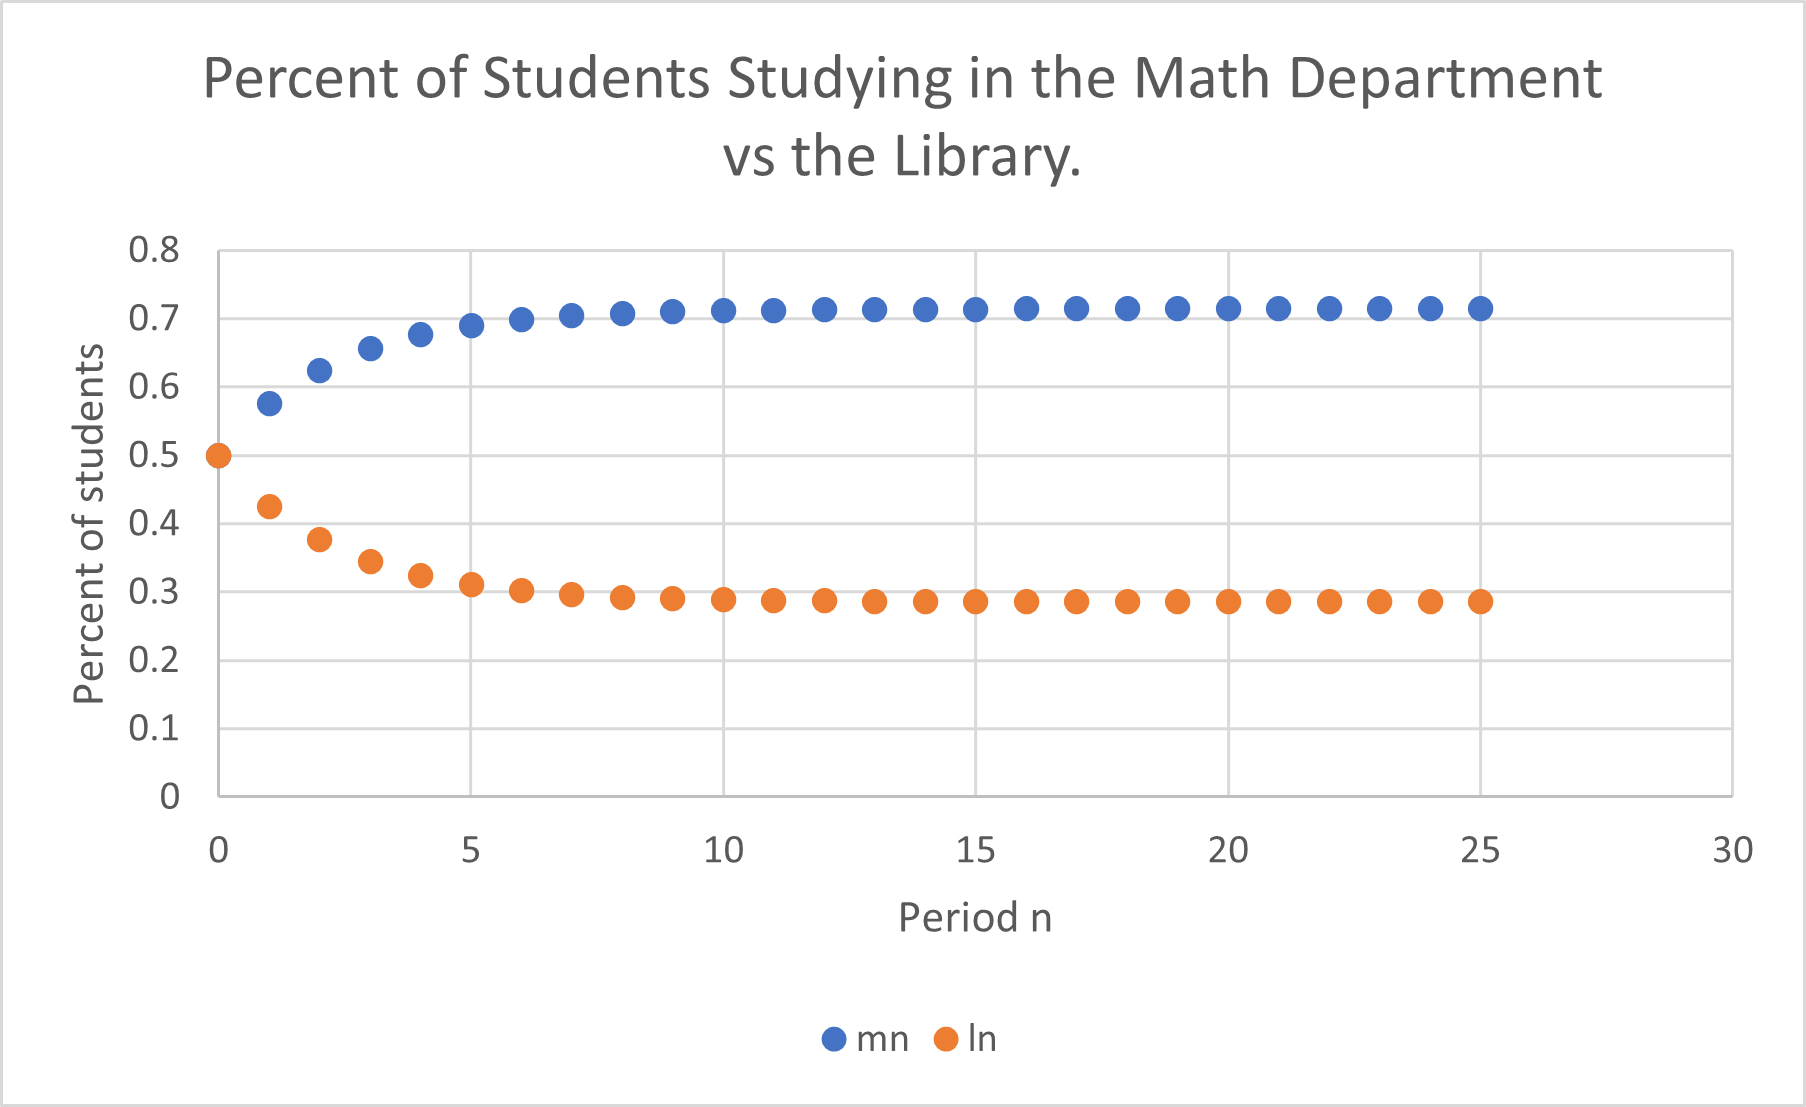
\includegraphics[scale=.8]{mn vs ln.png}}
  \caption{\label{fig:10} Plot of the percent of students in the math department vs the library}
\end{figure}

From our graph, we see the percent of students who study in the math department converges 
to a value around $.71$ or $71\%$ and those who study in the library converge to a value 
around $.29$ or $29\%$. We see this behavior with varying initial values in Figure \ref{fig:11} and \ref{fig:12} as well: 

\begin{figure}[!htb]
  \center{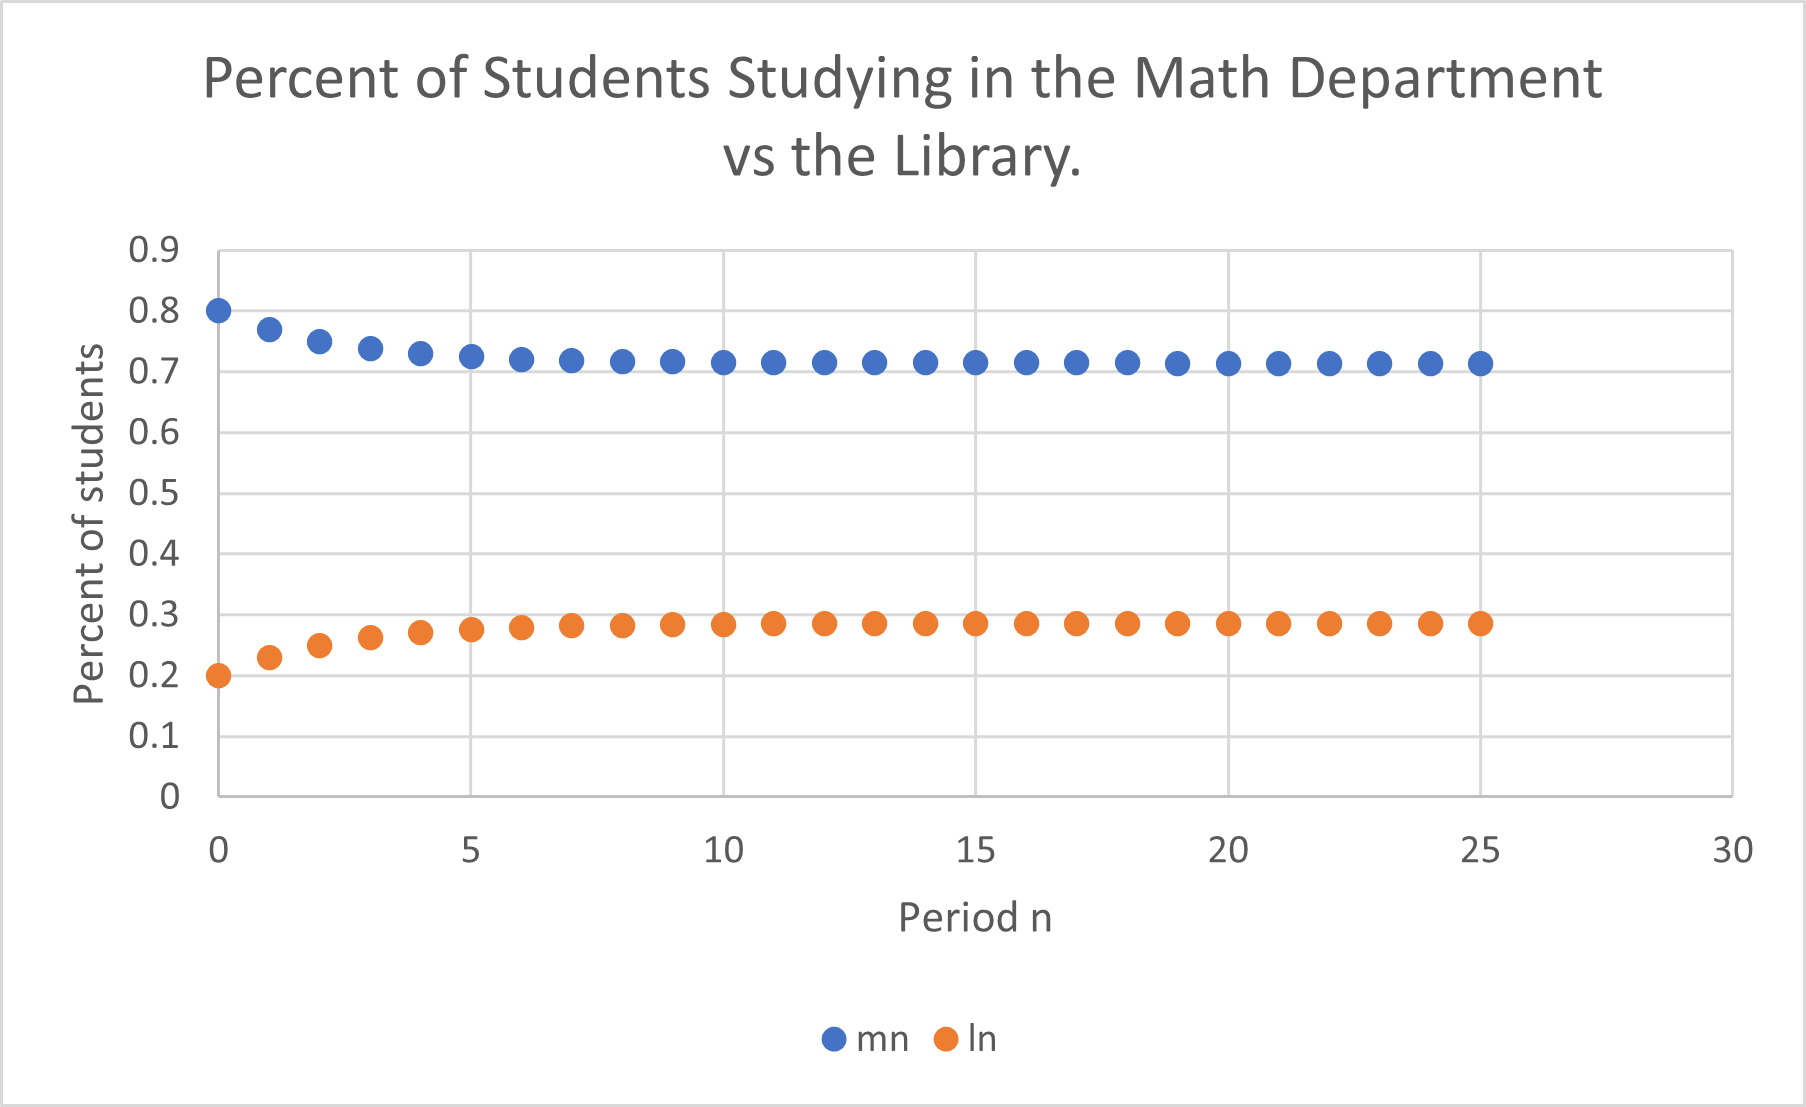
\includegraphics[scale=.8]{mn=.8 ln=.2.png}}
  \caption{\label{fig:11} Plot of the percent of students in the math department vs the library with $m_{0} = .8$ and $\ell_{0} = .2$}
\end{figure}

\begin{figure}[!htb]
  \center{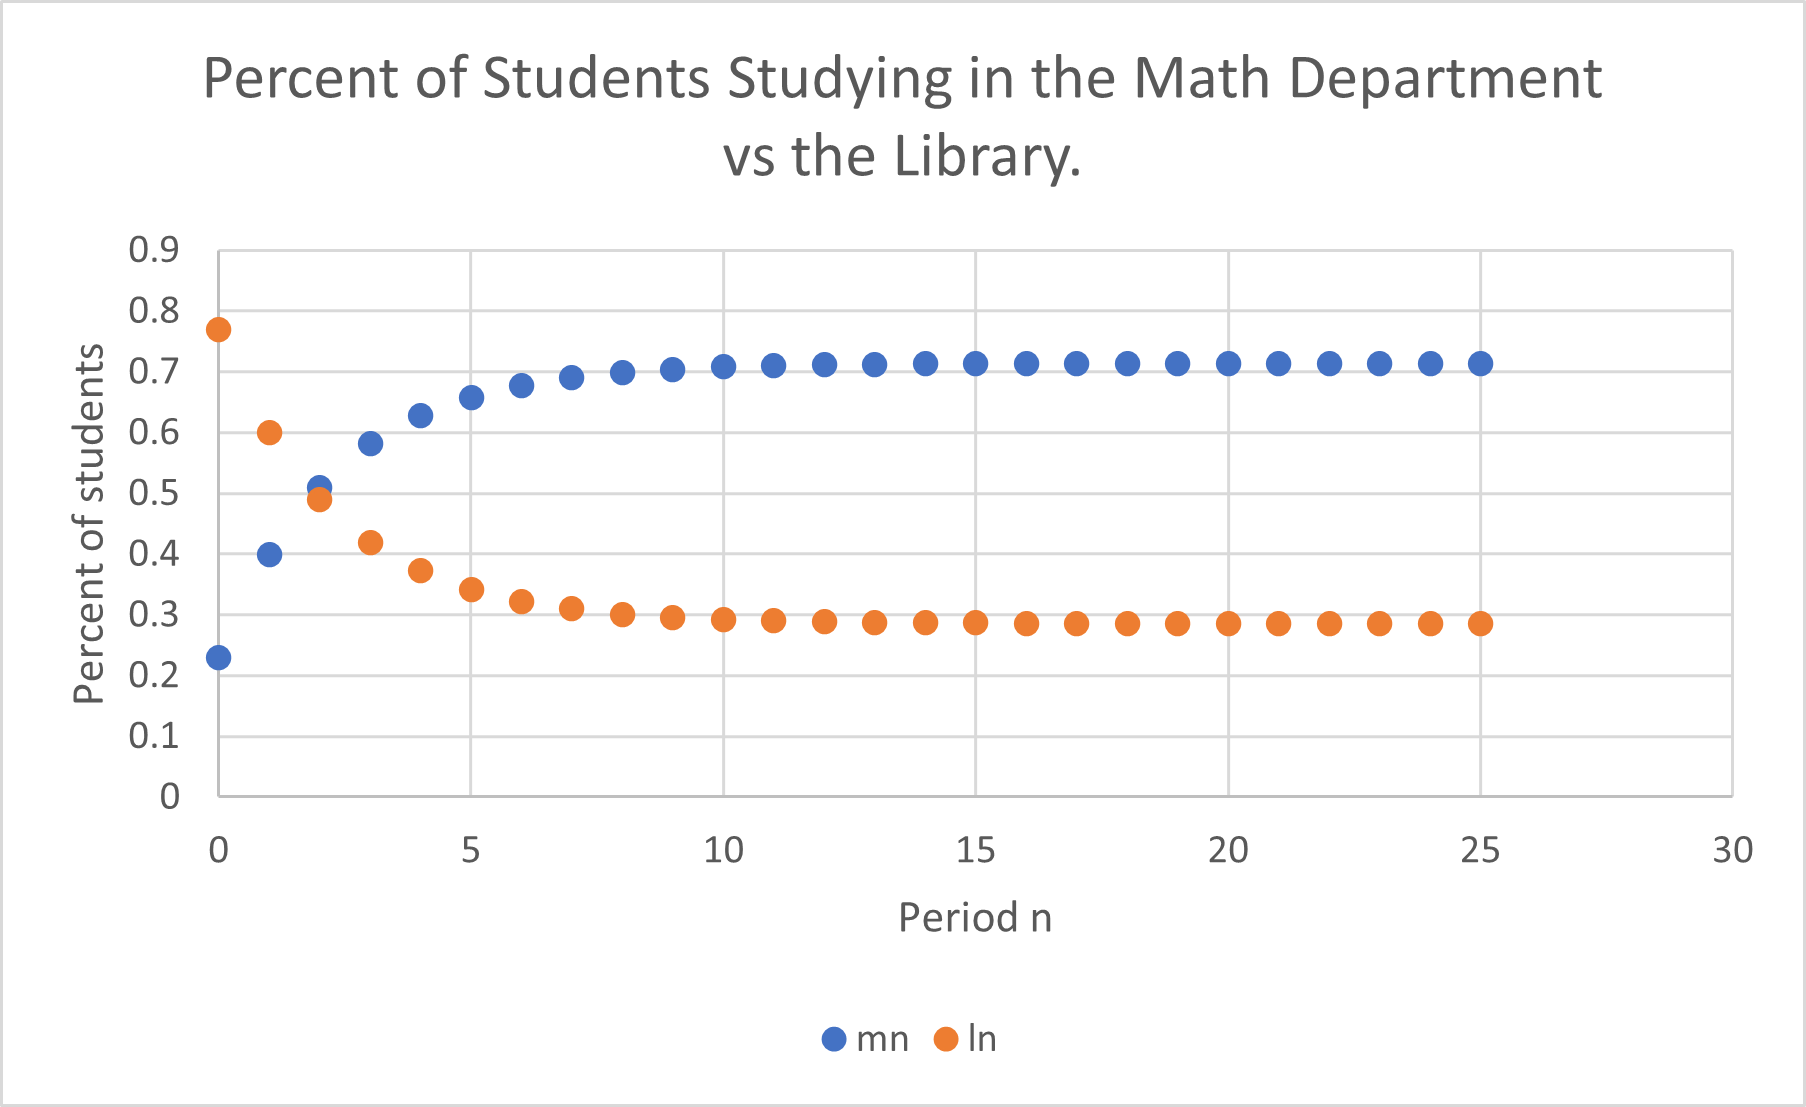
\includegraphics[scale=.8]{mn=.23 ln=.77.png}}
  \caption{\label{fig:12} Plot of the percent of students in the math department vs the library with $m_{0} = .8$ and $\ell_{0} = .2$}
\end{figure}
\vfill



\end{enumerate}


\end{document}